% This file was created with tikzplotlib v0.10.1.
\section{Changes in the years}
\label{Changes in the years}
Then the first thing that we have done is visualize the changes in the Expenditure of education based on the gross national income and government expenditure. 


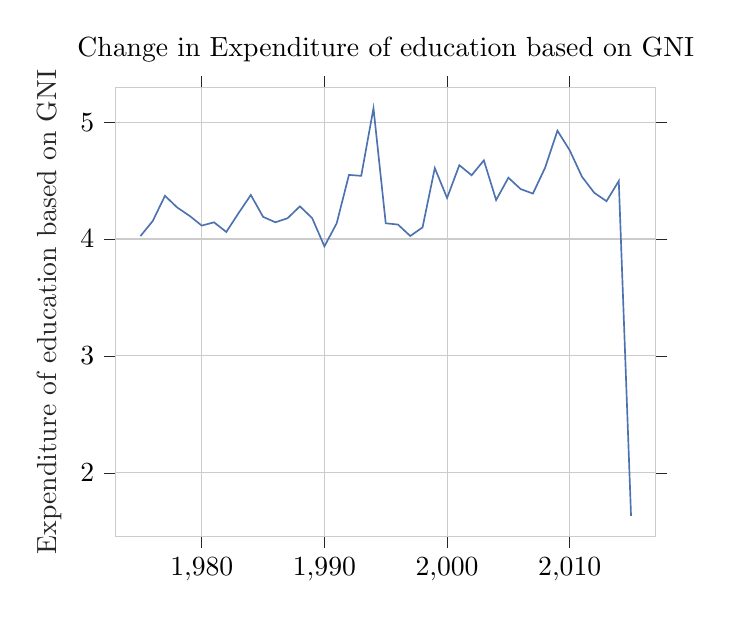
\begin{tikzpicture}

\definecolor{darkslategray38}{RGB}{38,38,38}
\definecolor{lightgray204}{RGB}{204,204,204}
\definecolor{steelblue76114176}{RGB}{76,114,176}

\begin{axis}[
axis line style={lightgray204},
tick align=outside,
title={Change in Expenditure of education based on GNI},
x grid style={lightgray204},
xmajorgrids,
xmajorticks=true,
xmin=1973, xmax=2017,
xtick style={color=darkslategray38},
y grid style={lightgray204},
ylabel=\textcolor{darkslategray38}{Expenditure of education based on GNI},
ymajorgrids,
ymajorticks=true,
ymin=1.45835584507042, ymax=5.29260725352113,
ytick style={color=darkslategray38}
]
\addplot [semithick, steelblue76114176]
table {%
1975 4.02496163636364
1976 4.153747
1977 4.3694866
1978 4.26920836734694
1979 4.19857392857143
1980 4.11477369230769
1981 4.14277701754386
1982 4.0604293442623
1983 4.22148836363636
1984 4.37679275862069
1985 4.18948236363636
1986 4.1431293442623
1987 4.17823218181818
1988 4.27948981818182
1989 4.17885403508772
1990 3.93714283018868
1991 4.13446909090909
1992 4.54812603448276
1993 4.54019810344828
1994 5.11832309859155
1995 4.13469780487805
1996 4.12349777777778
1997 4.02573473684211
1998 4.09935836956522
1999 4.60656366666667
2000 4.35107852459016
2001 4.63135483050847
2002 4.54524748031496
2003 4.67248342105263
2004 4.33330253968254
2005 4.52426238938053
2006 4.42712628318584
2007 4.38854252173913
2008 4.61147841269841
2009 4.92625675
2010 4.75855288
2011 4.53264247787611
2012 4.39545294736842
2013 4.3235108974359
2014 4.49612512195122
2015 1.63264
};
\end{axis}

\end{tikzpicture}
